% File: hawkdraw-doc.tex
% Copyright 2026 Jasper Habicht (mail(at)jasperhabicht.de).
%
% This work may be distributed and/or modified under the
% conditions of the LaTeX Project Public License version 1.3c,
% available at http://www.latex-project.org/lppl/.
%
% This file is part of the `hawkdraw' package (The Work in LPPL)
% and all files in that bundle must be distributed together.
%
% This work has the LPPL maintenance status `maintained'.
%
\DocumentMetadata{}
\documentclass[a4paper]{article}
\def\hawkdrawfileversion{0.2.0}
\def\hawkdrawfiledate{12 June 2026}

\usepackage[T1]{fontenc}
\usepackage{Alegreya}
\usepackage{AlegreyaSans}
\usepackage{FiraMono}

\usepackage{hawkdraw}

\usepackage{geometry, longtable, booktabs, siunitx, tcolorbox, hyperref}
\geometry{margin=25mm, left=45mm}
\DeclareSIUnit{\point}{pt}
\sisetup{detect-weight, detect-mode}
\urlstyle{same}

\usepackage{fancyhdr}
\pagestyle{fancy}
\fancyhf{}
\renewcommand{\headrulewidth}{0pt}
\fancyfoot[R]{\thepage}

\ExplSyntaxOn
\NewDocumentCommand{\fnstars}{m}{
  \int_step_inline:nn { \value{#1} } { * }
}
\ExplSyntaxOff

\linespread{1.1}\selectfont
\addtolength{\skip\footins}{1em plus 5pt}
\makeatletter
\renewcommand{\tableofcontents}{\@starttoc{toc}}
\renewcommand*{\thefootnote}{\fnstars{footnote}}
\renewcommand{\@makefnmark}{\normalfont\@thefnmark}
\renewcommand{\@makefntext}[1]{%
  \noindent\hbox to 1em{\normalfont\@thefnmark\hss}~#1%
}
\makeatother

\tcbuselibrary{skins,listings}
\lstdefinestyle{hawkdrawdocmacro}{
  basicstyle=\small\ttfamily,
  literate=*{<}{{{\color{black!50}\guilsinglleft}}}1
    {>}{{{\color{black!50}\guilsinglright}}}1,
  keywords={},
  moredelim=[is][\bfseries]{|}{|},
  moredelim=[is][\bfseries\itshape]{?}{?},
  moredelim=[is][\color{black!50}]{!}{!},
}
\lstdefinestyle{hawkdrawdocmacroalt}{
  basicstyle=\small\ttfamily,
  literate=*{<}{{{\color{black!50}\guilsinglleft}}}1
    {>}{{{\color{black!50}\guilsinglright}}}1,
  keywords={},
  moredelim=[is][\bfseries]{!}{!},
}
\lstdefinestyle{hawkdrawdoccodeexample}{
  basicstyle=\small\ttfamily,
  keywords={},
}

\hypersetup{colorlinks}

\ExplSyntaxOn
\int_new:N \l_hawkdraw_doc_change_int
\NewDocumentCommand{\changes}{ m m m }{
  \int_incr:N \l_hawkdraw_doc_change_int
  \prop_new:c { l_hawkdraw_doc_change_
    \int_to_roman:n { \l_hawkdraw_doc_change_int } _prop }
  \prop_put:cnn { l_hawkdraw_doc_change_
    \int_to_roman:n { \l_hawkdraw_doc_change_int } _prop } { version } {#1}
  \prop_put:cnn { l_hawkdraw_doc_change_
    \int_to_roman:n { \l_hawkdraw_doc_change_int } _prop } { date } {#2}
  \prop_put:cnn { l_hawkdraw_doc_change_
    \int_to_roman:n { \l_hawkdraw_doc_change_int } _prop } { changes } {#3}
}
\NewDocumentCommand{\printchanges}{ }{
  \section{Changes}
  \begin{description}
    \setlength\itemsep{0pt}
    \int_step_inline:nn { \l_hawkdraw_doc_change_int } {
      \item[
        \prop_item:cn { l_hawkdraw_doc_change_
        \int_to_roman:n { ##1 } _prop } { version } ~
        \normalfont{ (
          \prop_item:cn { l_hawkdraw_doc_change_
          \int_to_roman:n { ##1 } _prop } { date }
        ) }
      ]
      \prop_item:cn { l_hawkdraw_doc_change_
      \int_to_roman:n { ##1 } _prop } { changes }
    }
  \end{description}
}

\tl_new:N \l_hawkdraw_doc_doctitle_tl
\NewExpandableDocumentCommand{\makedoctitle}{ o m o m m o m }{
  \hypersetup{
    pdfauthor={#5},
    pdftitle={\IfValueTF{#1}{#1}{#2}},
    pdfsubject={\IfValueTF{#3}{#3}{#4}}
  }
  \tl_set:Nn \l_hawkdraw_doc_doctitle_tl {
    \group_begin:
      \tcbset{
        title ~ style ~ hook/.style={
          boxrule=2pt,
          fontupper=\huge\ttfamily
        }
      }
      \setlength{\parindent}{0pt}\sffamily
      \Huge{\bfseries #2}\par\bigskip
      \Large #4\par\bigskip
      \large #5
      \IfValueT{#6}{
        \,\footnote{#6}\par\bigskip
      }
      #7\par\bigskip
      \rule{\textwidth}{.08em}
    \group_end:
  }
}

\NewExpandableDocumentCommand{\printdoctitle}{ }{
  \tl_use:N \l_hawkdraw_doc_doctitle_tl
}
\ExplSyntaxOff

\NewDocumentCommand{\expandablestarcode}{ O{0,0} }{
  \fill[black!50, shift={([xshift={-10pt}, yshift={-10pt-0.5em}]#1)}]
    (90:3.75pt)
    \foreach \i in {1,...,4} {
      -- ({90+360/5*\i*2}:3.75pt)
    } -- cycle;
}

\NewDocumentCommand{\expandablestar}{}{
  \tikz{\expandablestarcode}
}

\NewDocumentCommand{\warning}{}{%
  \begin{tikzpicture}[overlay, baseline={(w.base)}]
    \node[circle, fill, black!25!red!10, text=black!25!red, outer sep=0pt]
      (w) at (-3em,0pt) {\bfseries !};
    \fill[black!25!red!10]
      (w.east) |- (w.south) -- cycle;
  \end{tikzpicture}%
}

\tcbset{
  size=small,
  arc=2.5pt,
  outer arc=2.5pt,
  colframe=black!10,
  colback=black!10,
  title style hook/.style={},
}

\NewTCBListing{macrodef}{ s o O{} }{
  listing only,
  listing style={hawkdrawdocmacro},
  grow to left by=2cm,
  boxrule=0pt,
  after={\par\smallskip\noindent},
  enhanced,
  IfValueT={#2}{
    hypertarget=#2
  },
  IfBooleanT={#1}{
    overlay={
      \expandablestarcode[frame.north east]
    }
  },
  #3
}

\NewTCBListing{codeexample}{ }{
  listing only,
  listing style={hawkdrawdoccodeexample},
  after={\par\smallskip\noindent}
}

\NewTCBListing{codeexamplecolumns}{ }{
  text side listing,
  lefthand width=2.5cm,
  listing style={hawkdrawdoccodeexample},
  after={\par\smallskip\noindent}
}

\NewTCBListing{macrodeprecated}{ s }{
  listing only,
  listing style={hawkdrawdocmacro},
  boxrule=0pt,
  width={0.5\linewidth-2.5pt},
  box align=top,
  after=\hfill,
  colframe=black!25!red!10,
  colback=black!25!red!10,
  enhanced,
  IfBooleanT={#1}{
    overlay={
      \fill[black!25!red!10]
        ([yshift={5pt-1.5em}]frame.north east)
        -- ++(5pt,-5pt) -- ++(-5pt,-5pt)
        -- cycle;
    }
  }
}

\NewTCBListing{macroreplacement}{ }{
  listing only,
  listing style={hawkdrawdocmacro},
  boxrule=0pt,
  width={0.5\linewidth-2.5pt},
  box align=top,
  before={},
  colframe=black!25!green!10,
  colback=black!25!green!10
}

\NewTotalTCBox{\macro}{ O{} v }{
  verbatim,
  size=tight,
  arc=1pt,
  outer arc=1pt,
  top=0.5pt,
  bottom=0.5pt,
  left=2pt,
  right=2pt,
  boxrule=0pt,
  colframe=black!10,
  colback=black!10,
  fontupper=\small\ttfamily,
  #1
}{\MathCollectFalse\vphantom{/g}\lstinline^#2^}

\NewTotalTCBox{\titlemacroinner}{ s O{} m }{
  verbatim,
  size=tight,
  arc=1pt,
  outer arc=1pt,
  top=0.5pt,
  bottom=0.5pt,
  left=2pt,
  right=2pt,
  boxrule=0pt,
  colframe=black!10,
  colback=black!10,
  fontupper=\small\ttfamily,
  title style hook,
  #2
}{\vphantom{/g}\IfBooleanT{#1}{\textbackslash}#3}

\NewDocumentCommand{\titlemacro}{ s O{} m }{%
  \IfBooleanTF{#1}{%
    \texorpdfstring{\titlemacroinner*[#2]{#3}}{#3}%
  }{%
    \texorpdfstring{\titlemacroinner[#2]{#3}}{#3}%
  }%
}

\usepackage{hawkdraw}

\makedoctitle
  [The hawkdraw package]
  {The \titlemacro{hawkdraw} package}
  {A LaTeX package to generate vector graphic output based on l3draw and related LaTeX3 modules using a simple syntax}
  {Jasper Habicht}[E-mail: \href{mailto:mail@jasperhabicht.de}{mail@jasperhabicht.de}. I am grateful to Joseph Wright, Max Chernoff, Clea F. Rees, Mikael Persson Sundqvist and Jonathan P. Spratte who helped me improving the code and the math behind it. Victor, the drawing hawk: \textcopyright{} 2026 Hannah Klöber.]
  {Version \hawkdrawfileversion, released on \hawkdrawfiledate}

\changes{v0.0.5}{2026/05/18}{First public alpha release.}
\changes{v0.0.6}{2026/05/20}{Splitting up code into modules.}
\changes{v0.0.7}{2026/05/25}{Adding patterns; adding \titlemacro{at part} option.}
\changes{v0.0.8}{2026/05/30}{Improving mapping functionality; adding mechanism to place arrow heads on paths; adding \titlemacro{at part} option for circles, ellipses and rectangles; adding \titlemacro{sloped} option for nodes; adding support for referencing anchors of nodes; adding possibility to reference points in calculations.}
\changes{v0.1.0}{2026/06/03}{Adding tagging support; adding basic intersection commands; adding plot functions; fixing node baseline anchors and slopes.}
\changes{v0.1.1}{2026/06/05}{Fixing bug in arrow tip slopes; fixing bugs in tagging support; improving option setting; adding option to set bounding box; adding ConTeXt module.}
\changes{v0.2.0}{2026/06/12}{Adding softpath system; improving ConTeXt module.}

\begin{document}
\vspace*{-1cm}
\noindent\hspace*{-3.5mm}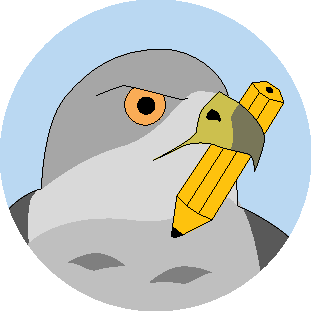
\includegraphics[width=5cm]{victor/victor.pdf}

\printdoctitle

\bigskip

\section{Introduction}

My sharp eyes spotted you, ground creature, already when you were still looking for this manual. Let me introduce myself: I am Victor, the drawing hawk. I epseically like drawing with LaTeX and since I value precision, using \macro{l3draw} in combination with \macro{l3fp} is my favourite way to draw. I created the \macro{hawkdraw} package to make it easier for you to use the powerful drawing capabilities of the LaTeX3 kernel.

The \macro{hawkdraw} package allows the user to use a simple syntax similar to Ti\emph{k}Z to generate vector graphic output based on \macro{l3draw} and related LaTeX3 modules such as \macro{l3fp} which provides very precise calculations. The syntax is meant to be simple and flexible but also coherent and logical with the aim of allowing the user to quickly draw graphics. The package name relates to the quickness and agility of hawks and the preciseness of their eyesight.

The package intends to define a set of user-level commands that can be used for drawing simple graphics. It does not aim to be a substitute for the Ti\emph{k}Z package or to offer a similar scope of application.

The package is currently still in an experimental stage. The code may be subject to fundamental and frequent changes. The author is grateful for reporting any bugs via GitHub at \url{https://github.com/jasperhabicht/hawkdraw/issues}. A site for asking questions about the package and for suggestions for improvement is available at \url{https://github.com/jasperhabicht/hawkdraw/discussions}.

\warning Note that the underlying code of the \macro{l3draw} package which is about to be included as module to the L3 kernel is experimental as well and hence might change possibly breaking the functionality of this package. Although a row of fall-backs exist to ensure backward compatibility, in order to ensure the functionality of the \macro{hawkdraw} package, it is highly recommended to use it with an up-to-date TeX distribution, especially with the most recent version of the \macro{l3draw} package.

\section{Contents}

\tableofcontents

\section{Loading the package}

To install the package, copy the package file \macro{hawkdraw.sty} together with the module files ending with \macro{.code.tex} into the working directory or into the \macro{texmf} directory. After the package has been installed, the \macro{hawkdraw} package is loaded by calling \macro{\usepackage{hawkdraw}} in the preamble of the document.

The package can be used with PDFLaTeX, LuaLaTeX or XeLaTeX. The package does not load any dependencies, but it needs a LaTeX kernel of 1 June 2022 or newer. It is recommended to use the package with an up-to-date TeX distribution.

\section{General remarks}

Similar to Ti\emph{k}Z, the \macro{hawkdraw} package makes use of key-value pairs to set options for commands. Some options are available for almost all commands, other have very specific uses. In the descriptions of the options, this manual states which data type the relevant option assumes. The following data types exist:

\begin{longtable}{ @{} p{2.5cm} p{\dimexpr\textwidth-2\tabcolsep-2.5cm} @{} }
  \toprule
  \textbf{Data type} & \textbf{Explanation} \\
  \midrule
  \macro{boolean} & A boolean only allows the values \macro{true} or \macro{false}. If not stated otherwise, setting the key without a value is equivalent with setting the key to \macro{true}. \\
  \macro{string} & A string is a concatenation of letters or numbers of any length. Typically, strings do not contain symbols. For example, strings are used for names of points, frames of nodes, patterns or arrow tips. \\
  \macro{float} & A floating-point number is a number without or with unit that uses a colon as decimal separator. \\
  \macro{dimension} & A dimension or length is a typical TeX length consisting of a floating point number and a length unit. \\
  \macro{tuple} & A tuple consists of two floating-point numbers without or with unit that are separated by a comma. A tuple may be enclosed by parenthesis. \\
  \macro{point} & A point is essentially a tuple, but it can also be a reference to a named node or, using a special syntax, denote a point in polar coordinates (see \hyperlink{sec:points}{below}). \\
  \macro{clist} & A comma-separated list is a list of strings that are separated by commas. Such a list can cosnist of no or only one item as well. If the relevant list can only have a maximum number of items, this is stated in the description of the relevant key. Note that a comma-separated list is typically not surrounded by parenthesis. \\
  \macro{options} & A key-value list consists of comma separated entities of keys that may be followed by an equals sign and a value. A value can be another key-value list. \\
  \macro{color} & This means a color definition as specified by the \macro{l3color} module. Note that colors defined by the \macro{xcolor} package have no effect when using the \macro{hawkdraw} package. \\
  \emph{none} & Some keys do not accept any data type as they are only executing some function. \\
  \bottomrule
\end{longtable}

Keys in the \macro{hawkdraw} package are divided into sets. Depending on where the keys are used in the document, only specific sets can be made use of. If a command or environment accepts specific sets of keys, the relevant prefix should be omitted.

\begin{macrodef}
|\hawkdrawset|{<options>}
\end{macrodef}
The command \macro{\hawkdrawset} is used to set options. It can be used inside or outside of \macro{hawkdraw} environments. It uses the \macro{path/} set of keys. If keys of other sets should be called, they need to be called from the root level.

For example keys of the \macro{picture/} set can be called using \macro{\hawkdrawset{picture/<key>}}.

\section{Main user environment}

\subsection{\titlemacro{hawkdraw} environment}

The package has only very few main user commands that can be used almost everywhere in the document body. Among these, the \macro{hawkdraw} environment is the most important as it is used to define a drawing and most other commands are only defined inside this environment.

\begin{macrodef}[env:hawkdraw]
\\\begin{|hawkdraw|}[<options>]
\end{|hawkdraw|}
\end{macrodef}
The \macro{hawkdraw} environment is the main environment for drawing. It defines most other commands described in the following sections. It can take an optional argument for options to the environment, which are explained in the following, or to paths which then apply to all paths inside the environment. As for options, the \macro{hawkdraw} environment accepts the \macro{picture/} set, the \macro{path/} set and the \macro{tag/} set.

\subsection{Setting baseline, layers and bounding box}

\begin{macrodef}
!picture/!|baseline|={<dimension>}
\end{macrodef}
The option \macro{baseline} sets the baseline for the environment as dimension. The default baseline is typically the bottom of the the bounding box of the drawing.

\begin{codeexamplecolumns}
foo
\begin{hawkdraw}[baseline={0pt}]
  \node[stroke, anchor={H,l}] {bar} ;
\end{hawkdraw}
baz
\end{codeexamplecolumns}

\begin{macrodef}[key:layers]
!picture/!|layers|={<clist>}
\end{macrodef}
The option \macro{layers} sets the layers for the environment as a comma-separated list. The layer \macro{main} must always be present and is the default layer. Layers are drawn in the order they are defined (see \hyperlink{sec:scopes}{below}).

\begin{macrodef}
!picture/!|bounding box|={auto}
!picture/!|bounding box|={zero}
!picture/!|bounding box|={<clist>}
!picture/!|overlay|
\end{macrodef}
The option \macro{bounding box} sets the environment to have a custom bounding box. It can take the value \macro{auto} which sets the bounding box to the default bounding box of the drawing. It can take the value \macro{zero} to set a zero-sized bounding box. It can also take as value a comma-separated list of four dimensions that define the lower left x- and y-coordinate as well as the upper right x- and y-coordinate of a rectangle that describes the bounding box of the drawing.

The option \macro{overlay} is an alias for \macro{bounding box={zero}}.

\begin{codeexamplecolumns}
foo
\begin{hawkdraw}[
  bounding box={zero},
  baseline={0pt}
] \stroke[color stroke={blue}]
    (0cm,0cm) circle[radius={0.5cm}] ;
\end{hawkdraw}
bar
\end{codeexamplecolumns}

Note that the \macro{hawkdraw} environment sets all category codes to the default LaTeX category codes, but it collects all characters with category code \num{13} (active) and a character code between \num{32} and \num{127}, resets these to active inside nodes and rescans the node's contents to ensure proper output.

\section{Scopes and layers}\label{sec:scopes}

\begin{macrodef}
\\\begin{|scope|}[<options>]
\end{|scope|}
\end{macrodef}
The \macro{scope} environment is only available inside the \macro{hawkdraw} environment. It can be used to create scopes for the localization of path states, style settings and clipping regions. As for options, the \macro{scope} environment accepts the \macro{scope/} set, the \macro{path/} set and the \macro{tag/} set.

\begin{codeexamplecolumns}
\begin{hawkdraw}[color fill={blue}]
  \fill (0cm,0cm) circle[radius={5pt}] ;
  \begin{scope}[color fill={black}]
    \fill (1cm,0cm) circle[radius={5pt}] ;
  \end{scope}
  \fill (2cm,0cm) circle[radius={5pt}] ;
\end{hawkdraw}
\end{codeexamplecolumns}

\begin{macrodef}
!scope/!|layer|={<string>}
\end{macrodef}
The option \macro{layer} sets the scope to be placed on the relevant layer. The layer must be defined beforehand using the \macro{layers} option (see \hyperref{key:layers}{above}).

\begin{codeexamplecolumns}
\begin{hawkdraw}[layers={background,main}]
  \fill[color fill={blue}]
    (0cm,0cm) circle[radius={0.5cm}] ;
  \begin{scope}[layer={background}]
    \fill (0.5cm,0cm) circle[radius={0.5cm}] ;
  \end{scope}
\end{hawkdraw}
\end{codeexamplecolumns}

\section{Path syntax}

\subsection{Path command and options}

\begin{macrodef}
|\path| <path operations> ;
\end{macrodef}
The command \macro{\path} is used to to draw a path inside the \macro{hawkdraw} environment. The path is defined by a sequence of points and path construction operations. Each \macro{\path} command must end with a semicolon. The following operations can be used to construct the path:

\begin{macrodef}
|[|<options>|]|
\end{macrodef}
Options can be for the path using square brackets. The command \macro{\path} accepts the \macro{path/} set including all subsets. Options can be set multiple times for the same path after any point on the path. Some options (such as color options or transformations) will apply to the entire path and the last specified value will be used.

\subsection{Points on the path}\label{sec:points}

Generally, the package makes use of the \macro{l3fp} module of the LaTeX kernel. As such, it is possible to execute calculations on the fly to define the points. The basic form of a point is a tuple of two expressions resulting in a floating-point number where both expressions are separated by a comma.

It is advisable to enclose the two expressions of the tuple in curly braces in cases where complicated calculations should be executed in order to create a group to ensure proper evaluation and avoiding conflicts with parsing the coordinates, especially when using a syntax for polar points as described below.

\begin{macrodef}
|(|<float>|,|<float>|)|
\end{macrodef}
Points on the path can be defined using x and y parts as floating-point numbers. The first item in the tuple is the x-coordinate, and the second item is the y-coordinate.

Points are per default defined as tuples representing the x- and y-coordinate. If floating-point numbers without unit are used, points are assumed per default. If other units are used, these are converted into points internally. The below alternative representations of points are as well calculated into the default tuple representation:

\begin{macrodef}
|(|<float>|>|<float|)|
|(|<float|,|<float>|>|<float>|)|
\end{macrodef}
Points on the path can also be defined using radius and angle parts as floating-point numbers. The first item in the tuple is the radius and the second item is the angle. The first item can contain a comma to define two radii.


\begin{macrodef}
|(|<float>|:|<float>|)|
|(|<float>|:|<float>|,|<float>|)|
\end{macrodef}
Points on the path can also be defined using radius and angle parts as floating-point numbers in reversed order. The first item in the tuple is the angle, and the second item is the radius. The seocnd item can contain a comma to define two radii.

\begin{macrodef}[macro:point]
|(|<string>|)|
\end{macrodef}
Points on the path can finally be referenced using names as strings. Points on the path can be named by either using the \macro{point} or the \macro{node} operation with the given name set via the \macro{nname} option (see \hyperlink{operation:point}{below}).

\subsection{Straight lines}

\begin{macrodef}
|--| (<point>)
\end{macrodef}
Using \macro{--} a line to the next point is drawn.

\begin{codeexamplecolumns}
\begin{hawkdraw}
  \path[stroke] (0cm,0cm)
    -- (2cm,1cm) ;
\end{hawkdraw}
\end{codeexamplecolumns}

\begin{macrodef}[][listing style={hawkdrawdocmacroalt}]
!|-! (<point>)
!-|! (<point>)
\end{macrodef}
Using \macro{|-} a vertical, then horizontal line to the next point is drawn. Using \macro{-|} a vertical, then horizontal line to the next point is drawn.

\begin{codeexamplecolumns}
\begin{hawkdraw}
  \path[stroke] (0cm,0cm)
    |- (2cm,1cm) ;
\end{hawkdraw}
\end{codeexamplecolumns}

\begin{codeexamplecolumns}
\begin{hawkdraw}
  \path[stroke] (0cm,0cm)
    -| (2cm,1cm) ;
\end{hawkdraw}
\end{codeexamplecolumns}

\subsection{Bézier curves}

\begin{macrodef}
|..| (<control point>) |..| (<point>)
|..| (<control point>) |&| (<control point>) |..| (<point>)
\end{macrodef}
The above syntax draws a Bézier curve to the next point with a single control point (quadratic Bézier) or with two control points (cubic Bézier).

\begin{codeexamplecolumns}
\begin{hawkdraw}
  \path[stroke] (0cm,0cm)
    .. (1cm,1cm)
    .. (2cm,1cm) ;
\end{hawkdraw}
\end{codeexamplecolumns}

\begin{codeexamplecolumns}
\begin{hawkdraw}
  \path[stroke] (0cm,0cm)
    .. (0cm,0.5cm) & (1cm,1cm)
    .. (2cm,1cm) ;
\end{hawkdraw}
\end{codeexamplecolumns}

\subsection{Closing paths}

\begin{macrodef}
|!|
\end{macrodef}
Using \macro{!} the path is closed by drawing a line from the last point to the first point.

\begin{codeexamplecolumns}
\begin{hawkdraw}
  \path[stroke] (0cm,0cm)
    -- (2cm,1cm)
    -- (0cm,1cm) ! ;
\end{hawkdraw}
\end{codeexamplecolumns}

\subsection{Circles, ellipses, arcs, rectangles and grids}

As for options, the following operators only accept the relevant subset to the \macro{path/} set.

\begin{macrodef}
|circle|[<options>]
\end{macrodef}
Using the \macro{circle} operation, a circle is drawn with the current point as center.

\begin{macrodef}
!path/circle/!|radius|={<dimension>}
\end{macrodef}
The radius is specified as a dimension with the \macro{radius} option.

\begin{codeexamplecolumns}
\begin{hawkdraw}
  \path[stroke] (0cm,0cm)
    circle[radius={1cm}] ;
\end{hawkdraw}
\end{codeexamplecolumns}

\begin{macrodef}
|ellipse|[<options>]
\end{macrodef}
Using the \macro{ellipse} operation, an ellipse is drawn with the current point as center.

\begin{macrodef}
!path/ellipse/!|radius x|={<dimension>}
!path/ellipse/!|radius y|={<dimension>}
!path/ellipse/!|vector a|={<tuple>}
!path/ellipse/!|vector b|={<tuple>}
\end{macrodef}
The vectors of the ellipse are specified as tuples of dimensions with the \macro{vector a} and \macro{vector b} options. ALternatively, the options \macro{radius x} and \macro{radius y} can be used to define the radii in the x- and y-dimension.

\begin{codeexamplecolumns}
\begin{hawkdraw}
  \path[stroke] (0cm,0cm)
    ellipse[
      radius x={0.5cm},
      radius y={1cm}
    ] ;
\end{hawkdraw}
\end{codeexamplecolumns}

\begin{codeexamplecolumns}
\begin{hawkdraw}
  \path[stroke] (0cm,0cm)
    ellipse[
      vector a={(0.5cm,1cm)},
      vector b={(0.75cm,0cm)}
    ] ;
\end{hawkdraw}
\end{codeexamplecolumns}

\begin{macrodef}
|arc|[<options>]
\end{macrodef}
Using the \macro{arc} operation, an arc is drawn with the current point as origin.

\begin{macrodef}
!path/arc/!|radius|={<dimension>}
!path/arc/!|radius x|={<dimension>}
!path/arc/!|radius y|={<dimension>}
!path/arc/!|vector a|={<tuple>}
!path/arc/!|vector b|={<tuple>}
!path/arc/!|angle start|={<float>}
!path/arc/!|angle end|={<float>}
!path/arc/!|angle delta|={<float>}
\end{macrodef}
The vectors of the arc are specified as tuples of dimensions with the options \macro{radius x} and \macro{radius y} that define the radii in the x- and y-dimension. It is possible to use the \macro{radius} option to define a uniform radius for both dimensions. Alternatively, the options \macro{vector a} and \macro{vector b} can be used to specify the vectors of the arc as tuples of dimensions. The angles are specified as dimensions with the \macro{angle start} and \macro{angle end} options. Instead of the \macro{angle end} option, the option \macro{angle delta} can be used.

\begin{codeexamplecolumns}
\begin{hawkdraw}
  \path[stroke] (0cm,0cm)
    arc[
      radius={1cm},
      angle start={45},
      angle end={135}
    ] ;
\end{hawkdraw}
\end{codeexamplecolumns}

\begin{codeexamplecolumns}
\begin{hawkdraw}
  \path[stroke] (0cm,0cm)
    arc[
      radius x={0.5cm},
      radius y={1cm},
      angle start={45},
      angle delta={90}
    ] ;
\end{hawkdraw}
\end{codeexamplecolumns}

\begin{codeexamplecolumns}
\begin{hawkdraw}
  \path[stroke] (0cm,0cm)
    arc[
      vector a={(0.5cm,1cm)},
      vector b={(0.75cm,0cm)},
      angle start={45},
      angle end={135}
    ] ;
\end{hawkdraw}
\end{codeexamplecolumns}

\begin{macrodef}
|rectangle|[<options>]
\end{macrodef}
Using the \macro{rectangle} operation, an rectangle with the current point as origin corner is drawn.

\begin{macrodef}
!path/rectangle/!|corner|={<tuple>}
!path/rectangle/!|relative|={<boolean>}
\end{macrodef}
The other corner of the rectangle is specified as a point (a tuple) with the \macro{corner} option. If the boolean option \macro{relative} is set, the corner point is interpreted as relative to the current point instead of absolute.

\begin{codeexamplecolumns}
\begin{hawkdraw}
  \path[stroke] (0cm,0cm)
    rectangle[corner={(2cm,1cm)}] ;
\end{hawkdraw}
\end{codeexamplecolumns}

\begin{macrodef}
|grid|[<options>]
\end{macrodef}
Using the \macro{grid} operation, a grid with the current point as origin corner is drawn.

\begin{macrodef}
!path/grid/!|step|={<clist>}
!path/grid/!|corner|={<tuple>}
!path/grid/!|relative|={<boolean>}
\end{macrodef}

The step is specified as a comma-separated list of at most two dimensions with the \macro{step} option. The first item in the list is the step in the x-direction, and the second item is the step in the y-direction. If only one dimension is given, it is used for both directions. The other corner is specified as a point (a tuple) with the \macro{corner} option. If the boolean option \macro{relative} is set, the corner point is interpreted as relative to the current point instead of absolute.

\begin{codeexamplecolumns}
\begin{hawkdraw}
  \path[stroke] (0cm,0cm)
    grid[step={10pt}, corner={(2cm,1cm)}] ;
\end{hawkdraw}
\end{codeexamplecolumns}

\begin{codeexamplecolumns}
\begin{hawkdraw}
  \path[stroke] (0cm,0cm)
    grid[step={5pt,10pt}, corner={(2cm,1cm)}] ;
\end{hawkdraw}
\end{codeexamplecolumns}

\subsection{Plot functions}

\begin{macrodef}
|plot|[<options>]{(<point>) ...}
\end{macrodef}
The \macro{plot} operator starts a path segment that uses a function as defined by the user. The operator initiates storing the last point and all points given in the braced argument in a sequence. After the operator, the function is executed using the points stored in the sequence. As for options, the \macro{plot} operator only accepts the \macro{path/plot/} subset.

\begin{macrodef}
!path/plot/!|function|={<string>}
\end{macrodef}

The plot function can be selected using the \macro{plot/function} key that expects the name of a plot function as string. Currently, two plot functions are predefined, \macro{sharp} and \macro{smooth}, the latter being selected per default. 

It is possible to use the \macro{map} operator inside the argument to the \macro{plot} operator.

\begin{codeexamplecolumns}
\begin{hawkdraw}
  \path[stroke, plot/function={smooth}] (0cm,0cm)
    plot {
      map[end=7] {
        ({#1 * 0.25cm},{sin(#1) * 0.25cm})
      } 
    }
  -- (1cm,1.5cm);
\end{hawkdraw}
\end{codeexamplecolumns}

\subsubsection{\titlemacro{sharp} plot function}

The \macro{sharp} plot function results in an output equivalent to the \macro{--} operator. It moves to the first point in the stored sequence and executes simple line-to operations to the following points.

\begin{codeexamplecolumns}
\begin{hawkdraw}
  \stroke[plot/function={sharp}] (0cm,0cm) 
    plot { (0.75cm,1cm) (1.5cm,.5cm) (2.25cm,.5cm) } ;
\end{hawkdraw}
\end{codeexamplecolumns}

\subsubsection{\titlemacro{smooth} plot function}

The \macro{smooth} plot function uses a simple algorithm to smoothen the curve. For paths that have more than three points, it takes the slope of a vector from the point before the relevant point to the point after the relevant point, scales this by a certain amount and uses the resulting points as control points for a Bézier curve. The first and the last path segments are quadratic Bézier curves, all other segments are cubic Bézier curves. If the path only contains two points, a straight line is drawn.

\begin{macrodef}
!path/plot/!|smooth/tension|={<float>}
\end{macrodef}

The factor by which the slope vector is scaled can be adjusted using the key \macro{plot/smooth/tension} which is set to \num{0.15} by default

\begin{codeexamplecolumns}
\begin{hawkdraw}
  \stroke[plot/function={smooth}] (0cm,0cm) 
    plot { (0.75cm,1cm) (1.5cm,.5cm) (2.25cm,.5cm) } ;
\end{hawkdraw}
\end{codeexamplecolumns}

\begin{codeexamplecolumns}
\begin{hawkdraw}
  \stroke[
    plot/function={smooth},
    plot/smooth/tension={0.25}
  ] (0cm,0cm) 
    plot { (0.75cm,1cm) (1.5cm,.5cm) (2.25cm,.5cm) } ;
\end{hawkdraw}
\end{codeexamplecolumns}

\subsection{Points and nodes}

Points are defined as tuple of two dimensions where the first represents the dimension on the x-axis and the second the dimension on the y-axis. Apart from defining points with these two dimensions directly, it is also possible to calculate these two dimensions or to define a point as being at a defined part of a path segment. Moreover, it is possible name points and later refer to them.

Nodes are boxes (coffins to be more exacct) that can contain arbitrary contents. Nodes also have frames that act as boxes surrounding these contents. Since such contents typically have some width and height, it is possible to refer to the corners and other points on the border of nodes via anchors.

\subsubsection{Points}

\begin{macrodef}[operation:point]
|point|[<options>]
\end{macrodef}
Using the \macro{point} operation, a point at the current position is defined and named with the given name. As for options, the \macro{point} operator only accepts the \macro{path/point/} subset.

\begin{macrodef}
!path/point/!|name|={<string>}
\end{macrodef}
The point can be referenced later by using the name in parentheses (see \hyperlink{macro:point}{above}).

The command \macro{\point} is a shortcut for \macro{\path (0pt,0pt) point}

\begin{codeexamplecolumns}
\begin{hawkdraw}
  \path (2cm,0.5cm) point[name={A}] ;
  \path[stroke] (0cm,0cm) -- (A) -- (0cm,1cm) ;
\end{hawkdraw}
\end{codeexamplecolumns}

\begin{macrodef}[key:atpart]
!path/point/!|at|={<tuple>}
!path/point/!|at part|={<float>}
!path/point/!|at distance|={<dimension>}
\end{macrodef}
The position of the point can be adjusted with the \macro{at} option which accepts a point (a tuple).

The position of a point can also be adjusted using the \macro{at part} option which accepts a floating-point number that defines the position on the last path segment with \num{0} being the previous and \num{1} being the current point. If the value given is negative or larger than \num{1}, the position of the point is interpolated according to the slope at the start or end of the path.

\begin{codeexamplecolumns}
\begin{hawkdraw}
  \stroke (0cm,0cm) -- (2cm,1cm)
    point[name={A}, at part={0.25}] ;
  \fill[color fill=red] (A) circle[radius={2pt}] ;
\end{hawkdraw}
\end{codeexamplecolumns}

Finally, the position of a point can be adjusted using the \macro{at distance} option which accepts a dimension that defines the position on the last path segment starting from the previous point. If the distance is negative or larger than the length of the path, the position of the point is interpolated according to the slope at the start or end of the path.

\begin{codeexamplecolumns}
\begin{hawkdraw}
  \stroke (0cm,0cm) -- (2cm,1cm)
    point[name={A}, at distance={30pt}] ;
  \fill[color fill=red] (A) circle[radius={2pt}] ;
\end{hawkdraw}
\end{codeexamplecolumns}

The position on a path using these options depend on the type of the path. For straight and curved lines as well as for circles and circular arcs, the distances are exact relative to the length of the path. For ellipses and elliptical arcs, the distances are distorted relative to the angle. For orthogonal lines, the distances are calculated such that half of the distance lies at the corner. For rectangles, the distances are calculated such that each side takes a quarter of the distance. The following examples show the output of different types of paths:

\begin{codeexamplecolumns}
\begin{hawkdraw}
  \path[stroke] (0cm,0cm)
    -- (2cm,1cm)
    point[name={A}, at part={0}]
    point[name={B}, at part={0.5}]
    point[name={C}, at part={0.9}] ;
  \fill[color fill=red] (A) circle[radius={2pt}] ;
  \fill[color fill=blue] (B) circle[radius={2pt}] ;
  \fill[color fill=green] (C) circle[radius={2pt}] ;
\end{hawkdraw}
\end{codeexamplecolumns}

\begin{codeexamplecolumns}
\begin{hawkdraw}
  \path[stroke] (0cm,0cm)
    -| (2cm,1cm)
    point[name={A}, at part={0}]
    point[name={B}, at part={0.5}]
    point[name={C}, at part={0.9}] ;
  \fill[color fill=red] (A) circle[radius={2pt}] ;
  \fill[color fill=blue] (B) circle[radius={2pt}] ;
  \fill[color fill=green] (C) circle[radius={2pt}] ;
\end{hawkdraw}
\end{codeexamplecolumns}

\begin{codeexamplecolumns}
\begin{hawkdraw}
  \path[stroke] (0cm,0cm)
    .. (1cm,1cm)
    .. (2cm,1cm)
    point[name={A}, at part={0}]
    point[name={B}, at part={0.5}]
    point[name={C}, at part={0.9}] ;
  \fill[color fill=red] (A) circle[radius={2pt}] ;
  \fill[color fill=blue] (B) circle[radius={2pt}] ;
  \fill[color fill=green] (C) circle[radius={2pt}] ;
\end{hawkdraw}
\end{codeexamplecolumns}

\begin{codeexamplecolumns}
\begin{hawkdraw}
  \path[stroke] (0cm,0cm)
    .. (0cm,0.5cm) & (1cm,1cm)
    .. (2cm,1cm)
    point[name={A}, at part={0}]
    point[name={B}, at part={0.5}]
    point[name={C}, at part={0.9}] ;
  \fill[color fill=red] (A) circle[radius={2pt}] ;
  \fill[color fill=blue] (B) circle[radius={2pt}] ;
  \fill[color fill=green] (C) circle[radius={2pt}] ;
\end{hawkdraw}
\end{codeexamplecolumns}

\begin{codeexamplecolumns}
\begin{hawkdraw}
  \path[stroke] (0cm,0cm)
    arc[
      radius={1cm},
      angle start={45},
      angle end={135}
    ]
    point[name={A}, at part={0}]
    point[name={B}, at part={0.5}]
    point[name={C}, at part={0.9}] ;
  \fill[color fill=red] (A) circle[radius={2pt}] ;
  \fill[color fill=blue] (B) circle[radius={2pt}] ;
  \fill[color fill=green] (C) circle[radius={2pt}] ;
\end{hawkdraw}
\end{codeexamplecolumns}

\begin{codeexamplecolumns}
\begin{hawkdraw}
  \path[stroke] (0cm,0cm)
    arc[
      vector a={(0.5cm,1cm)},
      vector b={(0.75cm,0cm)},
      angle start={45},
      angle end={135}
    ]
    point[name={A}, at part={0}]
    point[name={B}, at part={0.5}]
    point[name={C}, at part={0.9}] ;
  \fill[color fill=red] (A) circle[radius={2pt}] ;
  \fill[color fill=blue] (B) circle[radius={2pt}] ;
  \fill[color fill=green] (C) circle[radius={2pt}] ;
\end{hawkdraw}
\end{codeexamplecolumns}

\begin{codeexamplecolumns}
\begin{hawkdraw}
  \path[stroke] (0cm,0cm)
    circle[
      radius={1cm}
    ]
    point[name={A}, at part={0}]
    point[name={B}, at part={0.5}]
    point[name={C}, at part={0.9}] ;
  \fill[color fill=red] (A) circle[radius={2pt}] ;
  \fill[color fill=blue] (B) circle[radius={2pt}] ;
  \fill[color fill=green] (C) circle[radius={2pt}] ;
\end{hawkdraw}
\end{codeexamplecolumns}

\begin{codeexamplecolumns}
\begin{hawkdraw}
  \path[stroke] (0cm,0cm)
    ellipse[
      vector a={(0.5cm,1cm)},
      vector b={(0.75cm,0cm)}
    ]
    point[name={A}, at part={0}]
    point[name={B}, at part={0.5}]
    point[name={C}, at part={0.9}] ;
  \fill[color fill=red] (A) circle[radius={2pt}] ;
  \fill[color fill=blue] (B) circle[radius={2pt}] ;
  \fill[color fill=green] (C) circle[radius={2pt}] ;
\end{hawkdraw}
\end{codeexamplecolumns}

\begin{codeexamplecolumns}
\begin{hawkdraw}
  \path[stroke] (0cm,0cm)
    rectangle[
      corner={(2cm,1cm)}
    ]
    point[name={A}, at part={0}]
    point[name={B}, at part={0.5}]
    point[name={C}, at part={0.9}] ;
  \fill[color fill=red] (A) circle[radius={2pt}] ;
  \fill[color fill=blue] (B) circle[radius={2pt}] ;
  \fill[color fill=green] (C) circle[radius={2pt}] ;
\end{hawkdraw}
\end{codeexamplecolumns}

\begin{macrodef}*
|\getpoint|{<point>}
\end{macrodef}
Inside a \macro{hawkdraw} environment, the command \macro{\getpoint} can be used to access the coordinates of a point on the current path. The point is given as an argument. The command returns the coordinates of the point as a tuple of dimensions and can be used in subsequent calculations.

\begin{codeexamplecolumns}
\begin{hawkdraw}
  \point[name={A}, at={(1cm,1cm)}] ;
  \stroke[color stroke={blue}]
     (0cm,0cm) rectangle[corner={(A)}] ;
  \stroke (0cm,0cm)
    -- ({\getpoint{A} + (1cm,0cm)}) ;
\end{hawkdraw}
\end{codeexamplecolumns}

\begin{codeexamplecolumns}
\begin{hawkdraw}
  \point[name={A}, at={(1cm,0.5cm)}] ;
  \stroke[color stroke={blue}]
     (0cm,0cm) rectangle[corner={(A)}] ;
  \stroke (0cm,0cm)
    -- ({\getpoint{A} * 2}) ;
\end{hawkdraw}
\end{codeexamplecolumns}

\begin{codeexamplecolumns}
\begin{hawkdraw}
  \stroke (0cm,0cm)
    -- ({\getpoint{2cm>30}}) ;
\end{hawkdraw}
\end{codeexamplecolumns}

\begin{macrodef}*
|\getfirstpoint|
|\getlastpoint|
\end{macrodef}
The commands \macro{\getfirstpoint} and \macro{\getlastpoint} can be used to access the first and last point of the current path, respectively. The commands return the coordinates of the relevant point as a tuple of dimensions and can be used in subsequent calculations.

\begin{macrodef}*
|\getfirstslope|
|\getlastslope|
\end{macrodef}
The commands \macro{\getfirstslope} and \macro{\getlastslope} can be used to access the slope at the first and last point of the current path, respectively. The slope is represented as the angle with respect to the positive x-axis.

\begin{macrodef}*
|\getpointx|{<point>}
|\getpointy|{<point>}
\end{macrodef}
Inside a \macro{hawkdraw} environment, the commands \macro{\getpointx} and \macro{\getpointy} can be used to access the x- and y-coordinate of a point, respectively. The point is given as an argument, and the commands return the relevant coordinate as dimension.

\begin{macrodef}*
|\getpathlength|{<token list>}
\end{macrodef}
Inside a \macro{hawkdraw} environment, the command \macro{\getpathlength} retrieves the length of the current path (up to this point) and rstores this length as dimension in the token list given as argument.

\begin{macrodef}*
|\getintersectionlines|{<point>}{<point>}{<point>}{<point>}
\end{macrodef}
Inside a \macro{hawkdraw} environment, the command \macro{\getintersectionlines} can be used to access the intersection point of two lines. The lines are given as points in four arguments, the first two defining the first line and the last two defining the second line. The command returns the coordinates of the intersection point as a tuple of dimensions and can be used in subsequent calculations.

\begin{macrodef}*
|\getintersectioncircles|[<integer>]{<point>}{<dimension>}{<point>}{<dimension>}
\end{macrodef}
Inside a \macro{hawkdraw} environment, the command \macro{\getintersectioncircles} can be used to access the intersection points of two circles. The circles are given as a point and radius in the first and next two mandatory arguments. The optional argument specifies the number of the intersection to return (root) and defaults to \num{1}. The command returns the coordinates of the intersection points as tuples of dimensions and can be used in subsequent calculations.

\begin{macrodef}*
|\getintersectionlinecircle|[<integer>]{<point>}{<point>}{<point>}{<dimension>}
\end{macrodef}
Inside a \macro{hawkdraw} environment, the command \macro{\getintersectionlinecircle} can be used to access the intersection points of a line and a circle. The line is given as two points in the first two mandatory arguments, and the circle is given as a point and radius in the next two mandatory arguments. The optional argument specifies the number of the intersection to return (root) and defaults to \num{1}. The command returns the coordinates of the intersection points as tuples of dimensions and can be used in subsequent calculations.

\subsubsection{Nodes and frames}

\begin{macrodef}
|node|[<options>]{<content>}
\end{macrodef}
Using the \macro{node} operation, a node at the current position is defined and assigned the relevant content by the relevant argument. As for options, the \macro{node} operator accepts the \macro{path/node/} subset as well as the \macro{path/} set.

\begin{macrodef}
!path/node/!|rescan|={<boolean>}
\end{macrodef}
Using the \macro{rescan} option, the node's contents are rescanned using the current category ccodes. The default value is \macro{false}, but rescanning is activated automatically if active characters with character code between \num{32} and \num{127} are found before the relevant \macro{hawkdraw} environment.

\begin{macrodef}
!path/node/!|name|={<string>}
!path/node/!|at|={<tuple>}
!path/node/!|at part|={<float>}
!path/node/!|at distance|={<dimension>}
!path/node/!|anchor|={<clist>}
\end{macrodef}
The node can be named by setting the \macro{name} option which can be referenced later by using the name in parentheses (see \hyperlink{macro:point}{above}). Node names should not contain dots or dashes as these are reserved for referencing anchors. The position of the node can be adjusted with the \macro{at} option which accepts a point (a tuple) or with the options \macro{at part} or \macro{at distance} (see \hyperlink{key:atpart}{above}). The anchor is specified with the \macro{anchor} option which accepts a comma-separated list of at most two poles that define the anchor point as their intersection (see the explanations on coffins). Available poles are \macro{t}, \macro{b}, \macro{H} (which refers to the baseline of the node's contents), \macro{l}, \macro{r}, \macro{vc} and \macro{hc}. Nodes where the width is set additionally provide the poles \macro{T} and \macro{B} that refer to the top and bottom baseline of the node's contents respectively.

It is possible to reference a point where two poles of the node intersect by appending the node name with the relevant poles concatenated with a dash and separated by a dot from the node name. For example, if a node is named \macro{foo}, the point where the top and left pole of the node intersect can be referenced by \macro{(foo[t,l])}.

\begin{codeexamplecolumns}
\begin{hawkdraw}
  \node {foo} ;
\end{hawkdraw}
\end{codeexamplecolumns}

\begin{codeexamplecolumns}
\begin{hawkdraw}
  \node[stroke, name={A}] {foo} ;
  \fill[color fill=red] (A[b,l]) circle[radius={2pt}] ;
  \fill[color fill=red] (A[t,r]) circle[radius={2pt}] ;
\end{hawkdraw}
\end{codeexamplecolumns}

\begin{codeexamplecolumns}
\begin{hawkdraw}
  \stroke (0cm,0cm) -- (1cm,0.5cm)
    node[anchor={t,l}, stroke] {foo} ;
\end{hawkdraw}
\end{codeexamplecolumns}

\begin{macrodef}
!path/node/!|width|={<dimension>}
\end{macrodef}
The width of the node can be set with the \macro{width} option.

\begin{codeexamplecolumns}
\begin{hawkdraw}
  \stroke (0cm,0cm) -- (1cm,0.5cm)
    node[stroke, width={1cm}] {foo} ;
\end{hawkdraw}
\end{codeexamplecolumns}

\begin{macrodef}
!path/node/!|sloped|={<boolean>}
\end{macrodef}
Using the \macro{sloped} option, the node can be rotated to follow the direction of the path. The default value is \macro{false}.

\begin{codeexamplecolumns}
\begin{hawkdraw}
  \stroke (0cm,0cm) -- (2cm,1cm)
    node[
      stroke,
      at part={0.25},
      sloped
    ] {foo} ;
\end{hawkdraw}
\end{codeexamplecolumns}

\begin{macrodef}
!path/node/!|flipped|={<boolean>}
\end{macrodef}
Using the \macro{flipped} option, the node can be rotated by additional \num{180} degrees if it is sloped. The default value is \macro{false}.

\begin{macrodef}
!path/node/!|padding|={<clist>}
\end{macrodef}
Using the \macro{padding} option, the padding between the border of the node and the contents is set. The value is a comma-separated list of one to four dimensions. If four dimensions are given, they apply to the top, left, bottom and right side of the node respectively. If three dimensions are given, the first apples to the top, the second to the left and right side, the third to the bottom. If two dimensions are given, the first applies to the top and bottom and the second to the left and right sides. If only one dimension is given, it is appled to all four sides.

\begin{codeexamplecolumns}
\begin{hawkdraw}
  \node[
    stroke,
    at={(0cm,2cm)},
    padding={10pt}
  ] {foo} ;
  \node[
    stroke,
    at={(1.5cm,2cm)},
    padding={5pt,10pt}
  ] {foo} ;
  \node[
    stroke,
    at={(0cm,0cm)},
    padding={5pt,10pt,15pt}
  ] {foo} ;
  \node[
    stroke,
    at={(1.5cm,0cm)},
    padding={5pt,10pt,15pt,0pt}
  ] {foo} ;
\end{hawkdraw}
\end{codeexamplecolumns}

\begin{macrodef}
!path/node/!|color text|={<color>}
!path/node/!|opacity text|={<float>}
\end{macrodef}
Using the \macro{color text} option, the color of the node contents is set. The default text color is the current (text) color. The option \macro{text opacity} sets the text opacity. The floating-point number should be in the range of \num{0} and \num{1}. The default text opacity is \num{1} (fully opaque).

Note that \macro{\DocumentMetadata{}} needs to be set in order to activate support for PDF transparency.

\begin{macrodef}
!path/node/!|frame|={<string>}
\end{macrodef}
Using the \macro{frame} command, the frame surrounding the node text can be selected. The \macro{rectangle} frame is set per default. All options that are available for paths are also available for node frames.

\begin{codeexamplecolumns}
\begin{hawkdraw}
  \stroke (0cm,0cm) -- (1cm,0.5cm)
    node[
      fill, color fill={yellow},
      color text={blue},
      frame={ellipse}
    ] {foo} ;
\end{hawkdraw}
\end{codeexamplecolumns}

The command \macro{\node} is a shortcut for \macro{\path (0pt,0pt) node}

The following node frames are available, the frame \macro{none} is special as it removes the bounding box from the node altogether:

\NewDocumentCommand{\nodeframe}{ O{0.5ex} m }{%
  \begin{hawkdraw}[baseline={#1}]
    \path (-0.5cm,-0.25cm) rectangle[corner={(1cm,0.5cm)}] ;
    \node[frame={#2}, stroke] {foo} ;
  \end{hawkdraw}%
}

\begin{longtable}{ @{} p{2.5cm} p{\dimexpr\textwidth-2\tabcolsep-2.5cm} @{} }
  \toprule
  \textbf{Node frame} & \textbf{Name} \\
  \midrule
  \nodeframe{none} & \macro{none} \\
  \nodeframe{rectangle} & \macro{rectangle} \\
  \nodeframe{ellipse} & \macro{ellipse} \\
  \nodeframe{circle} & \macro{circle} \\
  \nodeframe{diamond} & \macro{diamond} \\
  \bottomrule
\end{longtable}

\section{Mapping operation}

\begin{macrodef}
|map|[<options>]{<code>}
\end{macrodef}
The \macro{map} operation is used to map over a comma-separated list of items or a range of numbers and execute code for each item that is given by the relevant argument. The code can reference the current item with \macro{#1} and the current index with \macro{#2}. The index starts at \num{1}. The \macro{map} operation can be nested. As for options, the \macro{map} operator only accepts the \macro{path/map/} subset.

\begin{macrodef}
!path/map/!|list|={<clist>}
!path/map/!|start|={<float>}
!path/map/!|end|={<float>}
!path/map/!|step|={<float>}
\end{macrodef}
The option \macro{list} sets the command to map over a comma-separated list of items. Each item in the list is passed as an argument to the code.

\begin{codeexamplecolumns}
\begin{hawkdraw}
  \fill
    map[list={30,150,270}] {
      (0.75cm>#1) circle[radius={5pt}]
    } ;
\end{hawkdraw}
\end{codeexamplecolumns}

The option \macro{start} sets the start of the range for mapping over a range of numbers as a floating-point number. The default start is \num{1}. The option \macro{end} sets the end of the range for mapping over a range of numbers as a floating-point number. The default end is \num{1}. The option \macro{step} sets the step for the range for mapping over a range of numbers as a floating-point number. The default step is \num{1}.

The command \macro{\map} is a shortcut for \macro{\path (0pt,0pt) map}

\begin{codeexamplecolumns}
\begin{hawkdraw}
  \map[start={30}, step={120}, end={270}] {
    [fill] (0.75cm>#1) circle[radius={5pt}]
  } ;
\end{hawkdraw}
\end{codeexamplecolumns}

\begin{codeexamplecolumns}
\begin{hawkdraw}
  \path[stroke]
    map[list={A,B}] {
      map[list={x,y}] {
        (#2 cm,##2 cm) node {#1,##1}
      }
    } ;
\end{hawkdraw}
\end{codeexamplecolumns}

\begin{codeexamplecolumns}
\begin{hawkdraw}
  \path[stroke] (0cm,0cm)
    .. (7mm,-10mm) & (14mm,8mm) .. (20mm,-5mm)
    map[end={10}] {
        tip[
          at part={0.095 * #1},
          color fill=blue! #1 0!red
        ] {stealth}
    } ;
\end{hawkdraw}
\end{codeexamplecolumns}

\begin{macrodef}
|\hawkdrawmap|[<option>]{<code>}
\end{macrodef}
The command \macro{\hawkdrawmap} can be used to repeat whole paths. The syntax is the same as for the \macro{map} opation.

\begin{macrodef}
|\hawkdrawarrayset|{<string>}{<clist>}
\end{macrodef}
The command \macro{\hawkdrawarrayset} can be used to define arrays of values. The first argument is the name of the array, and the second argument is a comma-separated list of items that are stored in the array. The items can be referenced with \macro{\hawkdrawarrayitem}.

\begin{macrodef}*
|\hawkdrawarrayitem|{<string>}{<integer>}
\end{macrodef}
The command \macro{\hawkdrawarrayitem} can be used to reference items in an array. The first argument is the name of the array, and the second argument is the index of the item to reference. The index is an integer where the first item has index \num{1}.

\begin{codeexamplecolumns}
\hawkdrawarrayset{myparts}{0,0.5,0.9}
\hawkdrawarrayset{mycolors}{red,blue,green}

\begin{hawkdraw}
  \path[stroke] (0cm,0cm)
    -- (2cm,1cm)
    map[list={A,B,C}] {
      point[
        name={#1},
        at part={\hawkdrawarrayitem{myparts}{#2}}
      ]
    } ;
  \hawkdrawmap[list={A,B,C}] {
    \fill[
      color fill={\hawkdrawarrayitem{mycolors}{#2}}
    ] (#1) circle[radius={2pt}] ;
  }
\end{hawkdraw}
\end{codeexamplecolumns}

\section{Path options}

The following options can be set for the path:

\subsection{Stroke and color fill, opacity, clipping}

\begin{macrodef}
!path/!|stroke|
!path/!|fill|
!path/!|clip|
\end{macrodef}
These options add a stroke to the path, fill the path, or use the path as a clipping region for subsequent paths. They can be used in combination. As the clipping region affects all following paths, it is often useful to use it in combination with scopes (see \hyperlink{sec:scopes}{above}).

The command \macro{\stroke} is a shortcut for \macro{\path [stroke]}.

The command \macro{\fill} is a shortcut for \macro{\path [fill]}.

The command \macro{\clip} is a shortcut for \macro{\path [clip]}.

\begin{codeexamplecolumns}
\begin{hawkdraw}
  \path[stroke, clip] (0cm,0cm)
    rectangle[corner={(2cm,1cm)}] ;
  \fill (1cm,0.5cm)
    circle[radius={0.6cm}] ;
\end{hawkdraw}
\end{codeexamplecolumns}

\begin{macrodef}
!path/!|color stroke|={<color>}
!path/!|color fill|={<color>}
!path/!|opacity stroke|={<float>}
!path/!|opacity fill|={<float>}
\end{macrodef}
The options \macro{color stroke} and \macro{color fill} set the color stroke and the color fill for the path. The default color stroke and color fill is the current (text) color.

\begin{codeexamplecolumns}
\begin{hawkdraw}[line width={5pt}]
  \path[
    fill, color fill={yellow},
    stroke, color stroke={blue}
  ] (0cm,0cm)
    rectangle[corner={(2cm,1cm)}] ;
\end{hawkdraw}
\end{codeexamplecolumns}

\begin{codeexamplecolumns}
\begin{hawkdraw}[line width={5pt}]
  \path[
    fill, opacity fill={0.25},
    stroke, opacity stroke={0.5}
  ] (0cm,0cm)
    rectangle[corner={(2cm,1cm)}] ;
\end{hawkdraw}
\end{codeexamplecolumns}

The options \macro{opacity stroke} and \macro{opacity fill} set the opacity stroke and the opacity fill for the path. The floating-point number should be in the range of \num{0} and \num{1}. The default opacity stroke and opacity fill is \num{1} (fully opaque).

Note that \macro{\DocumentMetadata{}} needs to be set in order to activate support for PDF transparency.

\subsection{Line styling}

\begin{macrodef}
!path/!|line width|={<dimension>}
\end{macrodef}
Sets the line width for the path. The default line width is \qty{0.4}{\point}.

\begin{codeexamplecolumns}
\begin{hawkdraw}
  \stroke
    (0cm,0cm) -- (2cm,1cm);
\end{hawkdraw}
\end{codeexamplecolumns}

\begin{codeexamplecolumns}
\begin{hawkdraw}
  \stroke[line width={5pt}]
    (0cm,0cm) -- (2cm,1cm) ;
\end{hawkdraw}
\end{codeexamplecolumns}

\begin{macrodef}
!path/!|line cap|={<string>}
!path/!|line join|={<string>}
!path/!|miter limit|={<float>}
\end{macrodef}
The option \macro{line cap} sets the line cap for the path. The possible values are \macro{butt}, \macro{round}, and \macro{rectangle}. The default line cap is \macro{butt}.

\begin{codeexamplecolumns}
\begin{hawkdraw}[line width={5pt}]
  \stroke[line cap={round}]
    (0cm,0cm) -- (2cm,1cm) ;
\end{hawkdraw}
\end{codeexamplecolumns}

The option \macro{line join} sets the line join for the path. The possible values are \macro{miter}, \macro{round}, and \macro{bevel}. The default line join is \macro{miter}.

The option \macro{miter limit} sets the miter limit for the path. The default miter limit is \num{10}.

\begin{codeexamplecolumns}
\begin{hawkdraw}[line width={5pt}]
  \stroke[line join={bevel}]
    (0cm,0cm) -- (2cm,0.5cm)
    -- (0cm,1cm) ;
\end{hawkdraw}
\end{codeexamplecolumns}

\begin{macrodef}
!path/!|dash pattern|={<clist>}
!path/!|dash phase|={<dimension>}
\end{macrodef}
The option \macro{dash pattern} sets the dash pattern for the path as a comma-separated list of dimensions. Each item in the list is a dimension representing the length of a dash or a gap. The default dash pattern is empty (a solid line).

The option \macro{dash phase} sets the dash phase for the path as a dimension. The default dash phase is \qty{0}{\point}.

\begin{codeexamplecolumns}
\begin{hawkdraw}
  \stroke[
    dash pattern={10pt,5pt},
    dash phase={2.5pt}
  ] (0cm,0cm) -- (2cm,1cm) ;
\end{hawkdraw}
\end{codeexamplecolumns}

\subsection{Rounded corners and fill rule}

\begin{macrodef}
!path/!|corner arc|={<clist>}
\end{macrodef}
The option \macro{corner arc} the corner arc for the path as a comma-separated list of at most two dimensions. The first applies to the corner formed by the path leading into the corner, and the second applies to the corner formed by the path leading out of the corner. If only one dimension is given, it applies to both corners. The default corner arc is \qty{0}{\point} (sharp corners).

\begin{codeexamplecolumns}
\begin{hawkdraw}
  \stroke[corner arc={5pt}] (0cm,0cm)
    rectangle[corner={(2cm,1cm)}] ;
\end{hawkdraw}
\end{codeexamplecolumns}

\begin{macrodef}
!path/!|fill rule|={<string>}
\end{macrodef}
This option sets the fill rule for the path. The possible values are \macro{non-zero} and \macro{even-odd}. The default fill rule is \macro{non-zero}. Note that this option is not influenced by scoping.

\begin{codeexamplecolumns}
\begin{hawkdraw}[fill rule={even-odd}]
  \fill (0cm,0cm)
    rectangle[corner={(2cm,1cm)}]
    (1cm,0.5cm)
    circle[radius={0.6cm}] ;
\end{hawkdraw}
\end{codeexamplecolumns}

\subsection{Transformations}

\begin{macrodef}
!path/!|shift|={<tuple>}
!path/!|rotate|={<float>}
!path/!|scale|={<tuple>}
!path/!|slant|={<tuple>}
\end{macrodef}
The option \macro{shift} sets the shift for the path as a tuple of dimensions. The first item in the tuple is the shift in the x-direction, and the second item is the shift in the y-direction. The default shift is (\qty{0}{\point}, \qty{0}{\point}).

\begin{codeexamplecolumns}
\begin{hawkdraw}
  \stroke[color stroke={blue}]
    (0cm,0cm) rectangle[corner={(2cm,1cm)}] ;
  \stroke[shift={(5pt,10pt)}]
    (0cm,0cm) rectangle[corner={(2cm,1cm)}] ;
\end{hawkdraw}
\end{codeexamplecolumns}

The option \macro{rotate} sets the rotation for the path as a floating-point number representing the angle of rotation. The default rotation is \qty{0}{\degree}.

\begin{codeexamplecolumns}
\begin{hawkdraw}
  \stroke[scale={0.25,0.5}]
    (0cm,0cm) rectangle[corner={(2cm,1cm)}] ;
\end{hawkdraw}
\end{codeexamplecolumns}

The option \macro{scale} sets the scale for the path as a comma-separated list of at most two floating-point numbers. The first item in the tuple is the scale in the x-direction, and the second item is the scale in the y-direction. If only one number is given, it is used for both directions. The default scale is (\num{1}, \num{1}).

\begin{codeexamplecolumns}
\begin{hawkdraw}
  \stroke[rotate={20}]
    (0cm,0cm) rectangle[corner={(2cm,1cm)}] ;
\end{hawkdraw}
\end{codeexamplecolumns}

The option \macro{slant} sets the slant for the path as a comma-separated list of at most two floating-point numbers. The first item in the tuple is the slant in the x-direction, and the second item is the slant in the y-direction. If only one number is given, it is used for both directions. The default slant is (\num{0}, \num{0}).

\begin{codeexamplecolumns}
\begin{hawkdraw}
  \stroke[slant={0.25,0.5}]
    (0cm,0cm) rectangle[corner={(2cm,1cm)}] ;
\end{hawkdraw}
\end{codeexamplecolumns}

\section{Path manipulations}

The packages makes use of a softpath mechanism that allows for manipulations of points of a paths. Currently, apart from rounding path corners via the \macro{corner arc} option which relies on a lower-level softpath implementation of \macro{l3draw}, only a mechanism for shortening paths is provided which is described below.

\section{Defining custom styles and colors}

\begin{macrodef}
!path/!|style set|={<options>}
!path/!|style add|={<options>}
\end{macrodef}
To simplify styling, custom keys can be defined via the keys \macro{style set} and \macro{style add}. Both keys accept as value a key-value list consisting of one or multiple custom keys whose relevant value consists of another key-value list describing the relevant style. It is possible to use \macro{#1} as placeholder for one argument. It is also possible to reference to an already define custom key in the definition of another custom key.

The key \macro{style set} defines custom keys and sets their values. The key \macro{style add} appends the relevant key-value list to the existing custom key as defined by \macro{style set}. Note that it is not checked whether a custom key already exists and its definition will be overwritten without a warning.

\begin{codeexamplecolumns}
\begin{hawkdraw}[
  style set={
    mystyle={
      stroke, color stroke={blue},
      line width={5pt}
    }
  }
]
  \path[mystyle]
    (0cm,0cm) -- (2cm,1cm) ;
\end{hawkdraw}
\end{codeexamplecolumns}

\begin{macrodef}
|\hawkdrawsetcolor|{<color>}{<model>}{<value>}
\end{macrodef}
The command \macro{\hawkdrawsetcolor} is used to define colors using the \macro{l3color} module. It is recommended to define custom colors in the preamble of the document. If the model is set to \macro{named}, the command expects as value a color expression.

\begin{codeexamplecolumns}
\hawkdrawsetcolor{colorA}{rgb}{0.1,0.5,0.8}
\hawkdrawsetcolor{colorB}{named}{yellow!90!red}
\begin{hawkdraw}[line width={5pt}]
  \path[
    stroke, color stroke={colorA},
    fill, color fill={colorB}
  ] (0cm,0cm) rectangle[corner={(2cm,1cm)}] ;
\end{hawkdraw}
\end{codeexamplecolumns}

\section{Arrow tips}

\subsection{Arrow tips at path ends}

\begin{macrodef}
!path/!|arrow start|={<string>}
!path/!|arrow end|={<string>}
\end{macrodef}
The options \macro{arrow start} and \macro{arrow end} set an arrow tip to the start and the end of the current path respectively. Both keys take as value a string representing the name of the relevant arrow tip. The \macro{default} arrow tip is selected per default. Arrow tips are not attached to single points or closed paths.

\begin{codeexamplecolumns}
\begin{hawkdraw}
  \stroke[arrow start, arrow end]
    (0cm,0cm) -- (2cm,1cm) ;
\end{hawkdraw}
\end{codeexamplecolumns}

\begin{macrodef}
!path/!|arrow style set|={<options>}
!path/!|arrow style add|={<options>}
!path/!|arrow start style set|={<options>}
!path/!|arrow start style add|={<options>}
!path/!|arrow end style set|={<options>}
!path/!|arrow end style add|={<options>}
\end{macrodef}
Arrow tips can be styled using the options \macro{arrow start style set} and \macro{arrow end style set}. The option \macro{arrow style set} sets the same style for start and end arrow tips.

The options \macro{arrow start style add}, \macro{arrow end style add} and \macro{arrow style add} append the relevant styles to the existing styles. All options that are available for paths are also available for arrow tips.

\begin{codeexamplecolumns}
\begin{hawkdraw}
  \stroke[
    arrow end,
    arrow style set={fill, color fill=blue}
  ]
    (0cm,0cm) -- (2cm,1cm) ;
\end{hawkdraw}
\end{codeexamplecolumns}

The following arrow tips are available, of these the last three, \macro{simple}, \macro{straight} and \macro{bar}, should be set together with the option \macro{arrow style set={stroke}}:

\NewDocumentCommand{\arrowexample}{ m }{%
  \begin{hawkdraw}[baseline={0.5ex}]
    \stroke[arrow end={#1}]
      (0cm,0cm) -- (1cm,0cm) ;
  \end{hawkdraw}%
}

\begin{longtable}{ @{} p{2.5cm} p{\dimexpr\textwidth-2\tabcolsep-2.5cm} @{} }
  \toprule
  \textbf{Arrow tip} & \textbf{Name} \\
  \midrule
  \arrowexample{none} & \macro{none} \\
  \arrowexample{default} & \macro{default} \\
  \arrowexample{stealth} & \macro{stealth} \\
  \arrowexample{triangle} & \macro{triangle} \\
  \arrowexample{circle} & \macro{circle} \\
  \arrowexample{simple} & \macro{simple} \\
  \arrowexample{straight} & \macro{straight} \\
  \arrowexample{bar} & \macro{bar} \\
  \bottomrule
\end{longtable}

\subsection{Arrow tips on paths}

\begin{macrodef}
|tip|[<options>] {<arrow>}
\end{macrodef}
Using the \macro{tip} operation, an arrow head is drawn at the current point on the path.

\begin{macrodef}
!path/tip/!|at part|={<float>}
!path/tip/!|at distance|={<dimension>}
\end{macrodef}
The position of the arrow head can be adjusted with the \macro{at part} option which accepts a unit-less floating-point number between \num{0} and \num{1} representing the position on the path or with the \macro{at distance} option which accepts a dimension (see \hyperlink{key:atpart}{above}).

\begin{codeexamplecolumns}
\begin{hawkdraw}
  \stroke (0cm,0cm) -- (2cm,1cm)
    tip[at part={0.25}] {straight} ;
\end{hawkdraw}
\end{codeexamplecolumns}

\begin{macrodef}
!path/tip/!|flipped|={<boolean>}
\end{macrodef}
If the boolean option \macro{flipped} is set, the arrow head is rotated to the other direction.

\begin{codeexamplecolumns}
\begin{hawkdraw}
  \stroke (0cm,0cm) -- (2cm,1cm)
    tip[at part={0.25}, flipped] {straight} ;
\end{hawkdraw}
\end{codeexamplecolumns}

\section{Patterns}

Note that in order to be able to use patterns, \macro{\DocumentMetadata{}} needs to be set.

\begin{macrodef}
!path/!|fill pattern|={<string>}
\end{macrodef}
The option \macro{fill pattern} sets a fill pattern for the current path. The key takes as value a string representing the name of the relevant pattern.

\begin{macrodef}
!path/!|pattern style set|={<options>}
!path/!|pattern style add|={<options>}
\end{macrodef}
Patterns can be styled using the options \macro{pattern style set} and \macro{pattern style add}. The option \macro{pattern style set} sets the style for the pattern of the current path. The options \macro{pattern style add} appends the relevant styles to the existing styles. All options that are available for paths are also available for patterns.

\begin{macrodef}
!path/!|pattern x|={<dimension>}
!path/!|pattern y|={<dimension>}
\end{macrodef}
The options \macro{pattern x} and \macro{pattern y} set the dimensions of the pattern in the x and y directions, respectively. The default dimensions of a pattern in both directions are both \qty{10}{\point}.

\begin{codeexamplecolumns}
\begin{hawkdraw}
  \path[
    fill pattern={dots},
    pattern style set={color fill=blue}
  ]
    (0cm,0cm) rectangle[corner={(2cm,1cm)}] ;
\end{hawkdraw}
\end{codeexamplecolumns}

The following patterns are available:

\NewDocumentCommand{\patternexample}{ m }{%
  \begin{hawkdraw}[baseline={0.5ex}]
    \path[fill pattern={#1}]
      (0cm,0cm) rectangle[corner={(2cm,1cm)}] ;
  \end{hawkdraw}%
}

\begin{longtable}{ @{} p{2.5cm} p{\dimexpr\textwidth-2\tabcolsep-2.5cm} @{} }
  \toprule
  \textbf{Pattern} & \textbf{Name} \\
  \midrule
  \patternexample{lines} & \macro{lines} \\
  \patternexample{hatch} & \macro{hatch} \\
  \patternexample{dots} & \macro{dots} \\
  \bottomrule
\end{longtable}

\section{Tagging support}

The \macro{hawkdraw} package supports tagging to provide accessible PDF structures. The following tags are available for the \macro{hawkdraw} environment as well as for nodes:

\begin{macrodef}
!tag/!|text|
!tag/!|artifact|
!tag/!|actualtext|={<string>}
!tag/!|alt|={<string>}
!tag/!|off|
\end{macrodef}
The \macro{text} key, which is set per default, tags all paths of a \macro{hawkdraw} environment as artifacts and the contents of all nodes as text in the order of their appearance in the code.

The option \macro{artifact} tags all paths and nodes of a \macro{hawkdraw} environment as artifact.

The option \macro{actualtext} sets the relevant value as replacement text for the \macro{hawkdraw} environment and tags it as inline span element.

The option \macro{alt} sets the relevant value as replacement text for the \macro{hawkdraw} environment and tags it as block (figure) element.

The option \macro{off} turns off tagging for the \macro{hawkdraw} environment.

\begin{macrodef}
!tag/!|tagging-setup|={<options>}
\end{macrodef}
To enable more complex tagging scenarios, the \macro{tagging-setup} option can be used to configure the tagging behavior. It accepts as options the same options as described above. In addition, it accepts the option \macro{tag} to define the element tag.

For example, the setting \macro{tagging-setup={alt={Water (H20)}, tag={Formula}}} would tag the \macro{hawkdraw} environment as a block element with the tag \macro{Formula} and set the replacement text to ``Water (H20)''.

\section{Use with ConTeXt}

The package provides a ConTeXt module that acts as a wrapper around the LaTeX package. The module loads PDFLaTeX from within ConTeXt to create a stand-alone PDF file from the relevant drawing that is then included into the ConTeXt document. To load the module in ConTeXt, call \macro{\usemodule[hawkdraw]}. 

\begin{macrodef}
|\starthawkdraw|[<options>]
|\stophawkdraw|
\end{macrodef}

The drawing code can the be used between the commands \macro{\starthawkdraw} and \macro{\stophawkdraw}.

\begin{codeexample}
\usemodule[hawkdraw]

\starttext
  \starthawkdraw
    \path[stroke] (0cm,0cm) -- (2cm,1cm) ;
  \stophawkdraw
\stoptext
\end{codeexample}

The \macro{\starthawkdraw} command can take options as argument. All options that are allowed for \macro{\setupframed} can be used. Also, the option \macro{options} can be used to pass options as described \hyperlink{env:hawkdraw}{above} for the \macro{hawkdraw} environment. For example, the below code can be used to set layers:

\begin{codeexample}
\starthawkdraw[options={layers={background,main}}]
  \fill[color fill={blue}]
    (0cm,0cm) circle[radius={0.5cm}] ;
  \begin{scope}[layer={background}]
    \fill (0.5cm,0cm) circle[radius={0.5cm}] ;
  \end{scope}
\stophawkdraw
\end{codeexample}

\begin{macrodef}
|\setuphawkdraw|[<options>]
\end{macrodef}

Instead of locally passing options to the \macro{\starthawkdraw} command, it is also possible to pass options to the \macro{\setuphawkdraw} command.

% =====

\printchanges

\end{document}